\documentclass[]{article}
\usepackage{lmodern}
\usepackage{amssymb,amsmath}
\usepackage{ifxetex,ifluatex}
\usepackage{fixltx2e} % provides \textsubscript
\ifnum 0\ifxetex 1\fi\ifluatex 1\fi=0 % if pdftex
  \usepackage[T1]{fontenc}
  \usepackage[utf8]{inputenc}
\else % if luatex or xelatex
  \ifxetex
    \usepackage{mathspec}
  \else
    \usepackage{fontspec}
  \fi
  \defaultfontfeatures{Ligatures=TeX,Scale=MatchLowercase}
\fi
% use upquote if available, for straight quotes in verbatim environments
\IfFileExists{upquote.sty}{\usepackage{upquote}}{}
% use microtype if available
\IfFileExists{microtype.sty}{%
\usepackage{microtype}
\UseMicrotypeSet[protrusion]{basicmath} % disable protrusion for tt fonts
}{}
\usepackage[margin=1in]{geometry}
\usepackage{hyperref}
\hypersetup{unicode=true,
            pdftitle={Making figures for RoM in R},
            pdfauthor={Max Lindmark},
            pdfborder={0 0 0},
            breaklinks=true}
\urlstyle{same}  % don't use monospace font for urls
\usepackage{color}
\usepackage{fancyvrb}
\newcommand{\VerbBar}{|}
\newcommand{\VERB}{\Verb[commandchars=\\\{\}]}
\DefineVerbatimEnvironment{Highlighting}{Verbatim}{commandchars=\\\{\}}
% Add ',fontsize=\small' for more characters per line
\usepackage{framed}
\definecolor{shadecolor}{RGB}{248,248,248}
\newenvironment{Shaded}{\begin{snugshade}}{\end{snugshade}}
\newcommand{\KeywordTok}[1]{\textcolor[rgb]{0.13,0.29,0.53}{\textbf{#1}}}
\newcommand{\DataTypeTok}[1]{\textcolor[rgb]{0.13,0.29,0.53}{#1}}
\newcommand{\DecValTok}[1]{\textcolor[rgb]{0.00,0.00,0.81}{#1}}
\newcommand{\BaseNTok}[1]{\textcolor[rgb]{0.00,0.00,0.81}{#1}}
\newcommand{\FloatTok}[1]{\textcolor[rgb]{0.00,0.00,0.81}{#1}}
\newcommand{\ConstantTok}[1]{\textcolor[rgb]{0.00,0.00,0.00}{#1}}
\newcommand{\CharTok}[1]{\textcolor[rgb]{0.31,0.60,0.02}{#1}}
\newcommand{\SpecialCharTok}[1]{\textcolor[rgb]{0.00,0.00,0.00}{#1}}
\newcommand{\StringTok}[1]{\textcolor[rgb]{0.31,0.60,0.02}{#1}}
\newcommand{\VerbatimStringTok}[1]{\textcolor[rgb]{0.31,0.60,0.02}{#1}}
\newcommand{\SpecialStringTok}[1]{\textcolor[rgb]{0.31,0.60,0.02}{#1}}
\newcommand{\ImportTok}[1]{#1}
\newcommand{\CommentTok}[1]{\textcolor[rgb]{0.56,0.35,0.01}{\textit{#1}}}
\newcommand{\DocumentationTok}[1]{\textcolor[rgb]{0.56,0.35,0.01}{\textbf{\textit{#1}}}}
\newcommand{\AnnotationTok}[1]{\textcolor[rgb]{0.56,0.35,0.01}{\textbf{\textit{#1}}}}
\newcommand{\CommentVarTok}[1]{\textcolor[rgb]{0.56,0.35,0.01}{\textbf{\textit{#1}}}}
\newcommand{\OtherTok}[1]{\textcolor[rgb]{0.56,0.35,0.01}{#1}}
\newcommand{\FunctionTok}[1]{\textcolor[rgb]{0.00,0.00,0.00}{#1}}
\newcommand{\VariableTok}[1]{\textcolor[rgb]{0.00,0.00,0.00}{#1}}
\newcommand{\ControlFlowTok}[1]{\textcolor[rgb]{0.13,0.29,0.53}{\textbf{#1}}}
\newcommand{\OperatorTok}[1]{\textcolor[rgb]{0.81,0.36,0.00}{\textbf{#1}}}
\newcommand{\BuiltInTok}[1]{#1}
\newcommand{\ExtensionTok}[1]{#1}
\newcommand{\PreprocessorTok}[1]{\textcolor[rgb]{0.56,0.35,0.01}{\textit{#1}}}
\newcommand{\AttributeTok}[1]{\textcolor[rgb]{0.77,0.63,0.00}{#1}}
\newcommand{\RegionMarkerTok}[1]{#1}
\newcommand{\InformationTok}[1]{\textcolor[rgb]{0.56,0.35,0.01}{\textbf{\textit{#1}}}}
\newcommand{\WarningTok}[1]{\textcolor[rgb]{0.56,0.35,0.01}{\textbf{\textit{#1}}}}
\newcommand{\AlertTok}[1]{\textcolor[rgb]{0.94,0.16,0.16}{#1}}
\newcommand{\ErrorTok}[1]{\textcolor[rgb]{0.64,0.00,0.00}{\textbf{#1}}}
\newcommand{\NormalTok}[1]{#1}
\usepackage{graphicx,grffile}
\makeatletter
\def\maxwidth{\ifdim\Gin@nat@width>\linewidth\linewidth\else\Gin@nat@width\fi}
\def\maxheight{\ifdim\Gin@nat@height>\textheight\textheight\else\Gin@nat@height\fi}
\makeatother
% Scale images if necessary, so that they will not overflow the page
% margins by default, and it is still possible to overwrite the defaults
% using explicit options in \includegraphics[width, height, ...]{}
\setkeys{Gin}{width=\maxwidth,height=\maxheight,keepaspectratio}
\IfFileExists{parskip.sty}{%
\usepackage{parskip}
}{% else
\setlength{\parindent}{0pt}
\setlength{\parskip}{6pt plus 2pt minus 1pt}
}
\setlength{\emergencystretch}{3em}  % prevent overfull lines
\providecommand{\tightlist}{%
  \setlength{\itemsep}{0pt}\setlength{\parskip}{0pt}}
\setcounter{secnumdepth}{0}
% Redefines (sub)paragraphs to behave more like sections
\ifx\paragraph\undefined\else
\let\oldparagraph\paragraph
\renewcommand{\paragraph}[1]{\oldparagraph{#1}\mbox{}}
\fi
\ifx\subparagraph\undefined\else
\let\oldsubparagraph\subparagraph
\renewcommand{\subparagraph}[1]{\oldsubparagraph{#1}\mbox{}}
\fi

%%% Use protect on footnotes to avoid problems with footnotes in titles
\let\rmarkdownfootnote\footnote%
\def\footnote{\protect\rmarkdownfootnote}

%%% Change title format to be more compact
\usepackage{titling}

% Create subtitle command for use in maketitle
\providecommand{\subtitle}[1]{
  \posttitle{
    \begin{center}\large#1\end{center}
    }
}

\setlength{\droptitle}{-2em}

  \title{Making figures for RoM in R}
    \pretitle{\vspace{\droptitle}\centering\huge}
  \posttitle{\par}
    \author{Max Lindmark}
    \preauthor{\centering\large\emph}
  \postauthor{\par}
      \predate{\centering\large\emph}
  \postdate{\par}
    \date{28 april 2019}

\usepackage{booktabs} \usepackage{longtable} \usepackage{array}
\usepackage{multirow} \usepackage[table]{xcolor} \usepackage{wrapfig}
\usepackage{float} \floatplacement{figure}{H}

\begin{document}
\maketitle

\subsection{Introduction}\label{introduction}

\subsubsection{Why R?}\label{why-r}

The main argument for using code to create RoM figures is to standardize
figures across species and to do so while limiting repetive work (you
only need to write a script once!). These figures here are made with the
package ggplot2, which is a very powerful tool for making multilevel
figures and allows for easy modification via the theme-function.

\subsubsection{Basic prerequisitis}\label{basic-prerequisitis}

It is an advantage if you know some Basic R. I strongly recommend using
R-studio and working in a so called R-studio project. When you open R,
click File/New Project/New Directory and specify where you want to save
it. Open the ``your\_project\_name''.Rproj and click File/New Script and
save that in your project folder. And that's it! The best thing is that
now all your search paths are relative and not absolute. If you want to
read in data, put the data inside the project folder and you don't have
to specify the full search path (``C:/R/RoM/data-file.csv''), it's
enought you give the name of the file only (more on that below!).
Another benefit with a relative search path is that I don't have to
worry about setting the working directory and changing the directory
each time I try to rerun anyone elses script.

Lastly, this is an R Markdown document. This means R-code is text with
grey background. You can copy these chunks of code to a new R-script in
your R-studio project.

\subsubsection{What does this script
do?}\label{what-does-this-script-do}

This script gives an example of how you can use R to create standardize
figures in R, and save them in a standardized resolution as a .tiff,
ready to be used without further editing.

I have chosen data for pike (\emph{Esox lucious}) as an example, because
it has all potential data for a RoM species (recreational, multiple
areas, error bars etc.). These data have been uploaded on github:
\url{https://github.com/maxlindmark/ROM}

\subsubsection{How do I use this for my
species?}\label{how-do-i-use-this-for-my-species}

Most basic RoM figures that all species have in some form can be grouped
into three different categories. Each category will have its own script.
Once you identify the best category for your species you \textbf{should
not have to modify the actual plotting code}, instead the aim to is to
only pre-define you vaiables. Do not worry! Instructions for how to do
that will be in the described below! The categories are:

\begin{itemize}
\tightlist
\item
  Fig. 1. Single series
\item
  Fig. 2. Multiple series
\item
  Fig. 3. Multiple series and y-axes
\end{itemize}

Check out the flowchart below to help identify which plot you need.

\begin{figure}
\centering
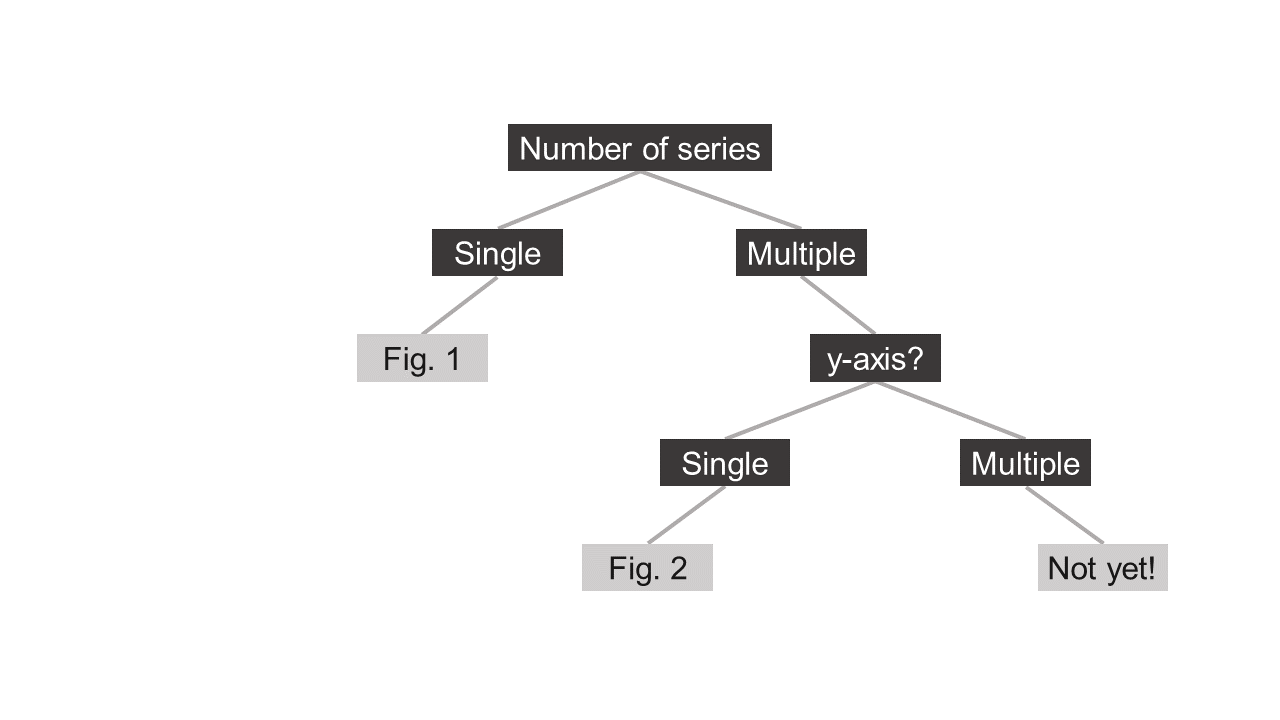
\includegraphics{Flow_chart.png}
\caption{How to select the best template for \textbf{your} species}
\end{figure}

Once you identify which plot type you will use, you can read about how
to prepare your data to use the script. A standardized way of saving
data is key for making any kind of standardized script! The data
structure is described in section \textbf{Preparation}.

This is a first draft and a work in progress so any feedback on this
document or the figures are highly appreciated!

\subsection{Preparation}\label{preparation}

\subsubsection{Load libraries}\label{load-libraries}

Before starting, we need to install a few packages:

\begin{Shaded}
\begin{Highlighting}[]
\KeywordTok{rm}\NormalTok{(}\DataTypeTok{list =} \KeywordTok{ls}\NormalTok{()) }\CommentTok{# clear the workspace from objects}

\CommentTok{# Provide package names}
\NormalTok{pkgs <-}\StringTok{ }\KeywordTok{c}\NormalTok{(}\StringTok{"devtools"}\NormalTok{, }\StringTok{"ggplot2"}\NormalTok{, }\StringTok{"RCurl"}\NormalTok{, }\StringTok{"RCurl"}\NormalTok{, }\StringTok{"tidyr"}\NormalTok{, }\StringTok{"dplyr"}\NormalTok{, }\StringTok{"scales"}\NormalTok{, }\StringTok{"png"}\NormalTok{, }\StringTok{"knitr"}\NormalTok{)}

\CommentTok{# Install packages}
\CommentTok{#install.packages(pkgs) # remove the hashtag if don't have them installed}

\CommentTok{# Load all packages}
\KeywordTok{invisible}\NormalTok{(}\KeywordTok{lapply}\NormalTok{(pkgs, }\ControlFlowTok{function}\NormalTok{(x) }\KeywordTok{require}\NormalTok{(x, }\DataTypeTok{character.only =}\NormalTok{ T, }\DataTypeTok{quietly =}\NormalTok{ T)))}
\end{Highlighting}
\end{Shaded}

\subsubsection{Load example data and clean it
up!}\label{load-example-data-and-clean-it-up}

Now let's read in the example data (freshwater pike):

\begin{Shaded}
\begin{Highlighting}[]
\CommentTok{# Go to https://github.com/maxlindmark/ROM to view the data in the browser}
\NormalTok{dat <-}\StringTok{ }\KeywordTok{read.csv}\NormalTok{(}
  \DataTypeTok{text =} \KeywordTok{getURL}\NormalTok{(}\StringTok{"https://raw.githubusercontent.com/maxlindmark/ROM/master/pike.csv"}\NormalTok{), }
  \DataTypeTok{sep =} \StringTok{";"}\NormalTok{)}
\end{Highlighting}
\end{Shaded}

For your own species, the code would typically look like this if you put
the data inside your R Project folder:

\begin{Shaded}
\begin{Highlighting}[]
\NormalTok{dat <-}\StringTok{ }\KeywordTok{read.csv}\NormalTok{(}\StringTok{"pike.csv"}\NormalTok{, }\DataTypeTok{sep =} \StringTok{";"}\NormalTok{)}
\end{Highlighting}
\end{Shaded}

Inspect the data:

\begin{Shaded}
\begin{Highlighting}[]
\KeywordTok{head}\NormalTok{(dat)}
\end{Highlighting}
\end{Shaded}

\begin{verbatim}
##   X.c5.r error rec_plus rec_minu        Omr.e5.de Ton
## 1   1997    NA       NA       NA Stora sj<f6>arna 115
## 2   1998    NA       NA       NA Stora sj<f6>arna 114
## 3   1999    NA       NA       NA Stora sj<f6>arna 149
## 4   2000    NA       NA       NA Stora sj<f6>arna 145
## 5   2001    NA       NA       NA Stora sj<f6>arna 121
## 6   2002    NA       NA       NA Stora sj<f6>arna 145
\end{verbatim}

Users will have different encoding which affects how certain characters
are read. Instead of forcing everyone to use the same encoding, I'm
showing you how to rename columns. It is \textbf{very} important that
you use these column names because they will determine which level gets
which colour and line (if you insist on other column names you have to
modify the plot code)!

\begin{Shaded}
\begin{Highlighting}[]
\NormalTok{dat <-}\StringTok{ }\NormalTok{dat }\OperatorTok\StringTok{ }\KeywordTok{rename}\NormalTok{(Områ}\DataTypeTok{de =}\NormalTok{ Omr.e5.de,}
\NormalTok{                      Å}\DataTypeTok{r     =}\NormalTok{ X.c5.r)}
\KeywordTok{head}\NormalTok{(dat)}
\end{Highlighting}
\end{Shaded}

\begin{verbatim}
##     År error rec_plus rec_minu           Område Ton
## 1 1997    NA       NA       NA Stora sj<f6>arna 115
## 2 1998    NA       NA       NA Stora sj<f6>arna 114
## 3 1999    NA       NA       NA Stora sj<f6>arna 149
## 4 2000    NA       NA       NA Stora sj<f6>arna 145
## 5 2001    NA       NA       NA Stora sj<f6>arna 121
## 6 2002    NA       NA       NA Stora sj<f6>arna 145
\end{verbatim}

Columns look better! But we also need to modify the actual levels of the
column (i.e.~the levels of the lakes). You can see which lakes are in
the data by typing:

\begin{Shaded}
\begin{Highlighting}[]
\KeywordTok{levels}\NormalTok{(dat}\OperatorTok{$}\NormalTok{Område)}
\end{Highlighting}
\end{Shaded}

\begin{verbatim}
## [1] "Fritidsfiske"     "Hj<e4>lmaren"     "M<e4>laren"      
## [4] "Stora sj<f6>arna" "V<e4>nern"        "V<e4>ttern"
\end{verbatim}

Clearly we also need to correct the names of the levels, similar to how
we did for column names. This is because the beauty of ggplot is that
all important information in the plot will be inherited from the data.

\begin{Shaded}
\begin{Highlighting}[]
\KeywordTok{levels}\NormalTok{(dat}\OperatorTok{$}\NormalTok{Område) <-}\StringTok{ }\KeywordTok{c}\NormalTok{(}\StringTok{"Fritidsfiske"}\NormalTok{, }
                        \StringTok{"Hjälmaren"}\NormalTok{, }
                        \StringTok{"Mälaren"}\NormalTok{, }
                        \StringTok{"Stora sjöarna"}\NormalTok{, }
                        \StringTok{"Vänern"}\NormalTok{, }
                        \StringTok{"Vättern"}\NormalTok{)}
\KeywordTok{head}\NormalTok{(dat)}
\end{Highlighting}
\end{Shaded}

\begin{verbatim}
##     År error rec_plus rec_minu        Område Ton
## 1 1997    NA       NA       NA Stora sjöarna 115
## 2 1998    NA       NA       NA Stora sjöarna 114
## 3 1999    NA       NA       NA Stora sjöarna 149
## 4 2000    NA       NA       NA Stora sjöarna 145
## 5 2001    NA       NA       NA Stora sjöarna 121
## 6 2002    NA       NA       NA Stora sjöarna 145
\end{verbatim}

There is one last thing you might need to do with the data before
proceeding with plotting, and that is to change the order of the levels
in the data. When plotting, ggplot sets the levels of the data in
alphabetical order, but here we want a specific order: the first
``level'' should correspond to the total and the last to any special
level, such as the recreational data.

\begin{Shaded}
\begin{Highlighting}[]
\NormalTok{dat}\OperatorTok{$}\NormalTok{Område <-}\StringTok{ }\KeywordTok{factor}\NormalTok{(dat}\OperatorTok{$}\NormalTok{Område,}
                     \DataTypeTok{levels =} \KeywordTok{c}\NormalTok{(}\StringTok{"Stora sjöarna"}\NormalTok{, }
                                \StringTok{"Vänern"}\NormalTok{, }
                                \StringTok{"Vättern"}\NormalTok{, }
                                \StringTok{"Mälaren"}\NormalTok{, }
                                \StringTok{"Hjälmaren"}\NormalTok{, }
                                \StringTok{"Fritidsfiske"}\NormalTok{))}
\end{Highlighting}
\end{Shaded}

Now the data look much better! You might not need to do these
modification on your own data. \textbf{But you need} to make sure it is
strutured in the same way, that is:

\begin{itemize}
\tightlist
\item
  1 row = 1 observation (not multiple columns for different areas)
\item
  first level (see last code chunk) corresponds to total biomass and
  last one is special series
\end{itemize}

\subsubsection{Define ggplot theme}\label{define-ggplot-theme}

Now that you have loaded and cleaned up your or the example data, we can
move on with general plotting settings. First the color palette:

\begin{Shaded}
\begin{Highlighting}[]
\NormalTok{pal <-}\StringTok{ }\KeywordTok{c}\NormalTok{(}\StringTok{"#56B4E9"}\NormalTok{, }\StringTok{"#009E73"}\NormalTok{, }\StringTok{"#F0E442"}\NormalTok{, }\StringTok{"#0072B2"}\NormalTok{, }\StringTok{"#E69F00"}\NormalTok{, }\StringTok{"#D55E00"}\NormalTok{)}
\end{Highlighting}
\end{Shaded}

Second, we define the theme we will use for all plots. This is made to
match as closely as possible to the RoM style. This applies to all
figures styles. In the future this function should be sourced but here I
show it in full. Make sure you copy paste this function and run it.

\begin{Shaded}
\begin{Highlighting}[]
\NormalTok{theme_rom <-}\StringTok{ }\ControlFlowTok{function}\NormalTok{(}\DataTypeTok{base_size =} \DecValTok{12}\NormalTok{, }\DataTypeTok{base_family =} \StringTok{""}\NormalTok{) \{}
  \KeywordTok{theme_bw}\NormalTok{(}\DataTypeTok{base_size =} \DecValTok{12}\NormalTok{, }\DataTypeTok{base_family =} \StringTok{""}\NormalTok{) }\OperatorTok{+}
\StringTok{    }\KeywordTok{theme}\NormalTok{(}
      \DataTypeTok{axis.text =} \KeywordTok{element_text}\NormalTok{(}\DataTypeTok{size =} \DecValTok{8}\NormalTok{), }
      \DataTypeTok{axis.title =} \KeywordTok{element_text}\NormalTok{(}\DataTypeTok{size =} \DecValTok{8}\NormalTok{),}
      \DataTypeTok{axis.ticks.length =} \KeywordTok{unit}\NormalTok{(}\FloatTok{0.05}\NormalTok{, }\StringTok{"cm"}\NormalTok{),}
      \DataTypeTok{axis.line =} \KeywordTok{element_line}\NormalTok{(}\DataTypeTok{colour =} \StringTok{"black"}\NormalTok{,}
                               \DataTypeTok{size =} \FloatTok{0.3}\NormalTok{), }
      \DataTypeTok{text =} \KeywordTok{element_text}\NormalTok{(}\DataTypeTok{family =} \StringTok{"sans"}\NormalTok{),}
      \DataTypeTok{panel.grid.major =} \KeywordTok{element_blank}\NormalTok{(),}
      \DataTypeTok{panel.grid.minor =} \KeywordTok{element_blank}\NormalTok{(),}
      \DataTypeTok{panel.border =} \KeywordTok{element_blank}\NormalTok{(),}
      \DataTypeTok{plot.title =} \KeywordTok{element_text}\NormalTok{(}\DataTypeTok{hjust =} \FloatTok{0.5}\NormalTok{, }
                                \DataTypeTok{margin =} \KeywordTok{margin}\NormalTok{(}\DataTypeTok{b =} \OperatorTok{-}\DecValTok{3}\NormalTok{), }
                                \DataTypeTok{size =} \FloatTok{9.6}\NormalTok{, }
                                \DataTypeTok{face =} \StringTok{"bold"}\NormalTok{),}
      \DataTypeTok{legend.position =} \KeywordTok{c}\NormalTok{(}\FloatTok{0.5}\NormalTok{, }\OperatorTok{-}\FloatTok{0.25}\NormalTok{),}
      \DataTypeTok{legend.text =} \KeywordTok{element_text}\NormalTok{(}\DataTypeTok{size =} \DecValTok{8}\NormalTok{),}
      \DataTypeTok{legend.justification =} \StringTok{"bottom"}\NormalTok{, }
      \DataTypeTok{legend.background =} \KeywordTok{element_rect}\NormalTok{(}\DataTypeTok{fill =} \StringTok{"transparent"}\NormalTok{), }
      \DataTypeTok{legend.key =} \KeywordTok{element_rect}\NormalTok{(}\DataTypeTok{fill =} \StringTok{"transparent"}\NormalTok{),}
      \DataTypeTok{aspect.ratio =} \DecValTok{1}\NormalTok{,}
      \DataTypeTok{plot.margin =} \KeywordTok{unit}\NormalTok{(}\KeywordTok{c}\NormalTok{(}\FloatTok{5.5}\NormalTok{, }\FloatTok{5.5}\NormalTok{, }\DecValTok{20}\NormalTok{, }\FloatTok{5.5}\NormalTok{), }
                         \StringTok{"points"}\NormalTok{)}
\NormalTok{      )}
\NormalTok{\}}
\end{Highlighting}
\end{Shaded}

\subsection{Let's start making
figures!}\label{lets-start-making-figures}

\subsection{Fig. 1. Single series}\label{fig.-1.-single-series}

\begin{figure}

{\centering 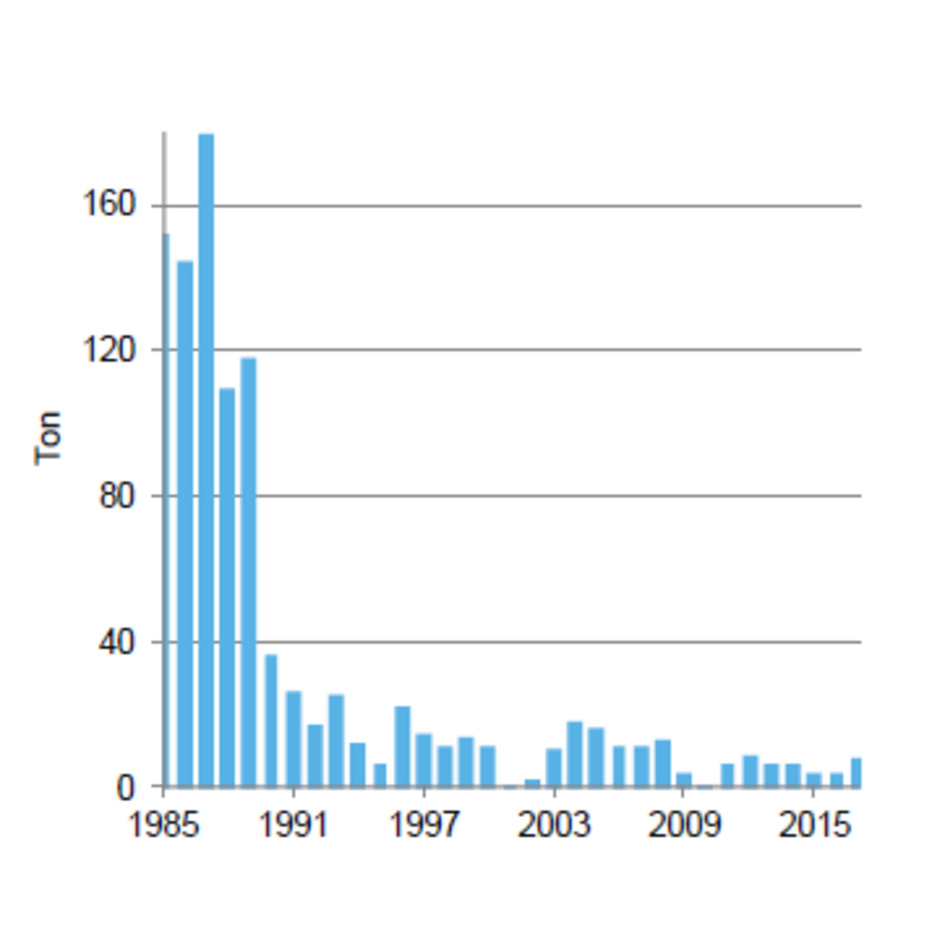
\includegraphics{sikloja} 

}

\caption{Siklöja in Mälaren (RoM 2018) - example of a single-series plot}\label{fig:unnamed-chunk-11}
\end{figure}

For illustration purposes, we will now pretend our example pike dataset
only is a single series, by filtering it to only contain the area
``Stora Sjöarna''. If you have Fig.1 situation, your data might look
something like this, with one column for year, one for area and one for
tonnes.

\begin{Shaded}
\begin{Highlighting}[]
\NormalTok{ dat1 <-}\StringTok{ }\NormalTok{dat }\OperatorTok\StringTok{ }
\StringTok{  }\KeywordTok{select}\NormalTok{(År, Ton, Område) }\OperatorTok\StringTok{ }
\StringTok{  }\KeywordTok{filter}\NormalTok{(Område }\OperatorTok{==}\StringTok{ "Stora sjöarna"}\NormalTok{)}
\end{Highlighting}
\end{Shaded}

We now need to specify y-axis titles and plot title. \textbf{This is
what is meant by predifing variables! Instead of changing the plotting
code we define what we want it to plot on the axis, for instance}. For
the pike data we can set them as:

\begin{Shaded}
\begin{Highlighting}[]
\NormalTok{y_axis <-}\StringTok{ }\KeywordTok{c}\NormalTok{(}\StringTok{"Landningar (ton)"}\NormalTok{)}
\NormalTok{title  <-}\StringTok{ }\KeywordTok{c}\NormalTok{(}\StringTok{"Landningar"}\NormalTok{)}
\end{Highlighting}
\end{Shaded}

Now go ahead and create the plot

\begin{Shaded}
\begin{Highlighting}[]
\NormalTok{p1 <-}\StringTok{ }\KeywordTok{ggplot}\NormalTok{(dat1, }\KeywordTok{aes}\NormalTok{(År, Ton)) }\OperatorTok{+}
\StringTok{  }\KeywordTok{geom_bar}\NormalTok{(}\DataTypeTok{data =}\NormalTok{ dat1, }
           \KeywordTok{aes}\NormalTok{(}\DataTypeTok{x =}\NormalTok{ År, }\DataTypeTok{y =}\NormalTok{ Ton), }\DataTypeTok{stat =} \StringTok{"identity"}\NormalTok{, }\DataTypeTok{color =}\NormalTok{ pal[}\DecValTok{1}\NormalTok{], }\DataTypeTok{fill =}\NormalTok{ pal[}\DecValTok{1}\NormalTok{], }
           \DataTypeTok{width =} \FloatTok{0.6}\NormalTok{) }\OperatorTok{+}
\StringTok{  }\CommentTok{#scale_color_manual(values = pal) +}
\StringTok{  }\KeywordTok{scale_alpha_manual}\NormalTok{(}\DataTypeTok{values =} \KeywordTok{c}\NormalTok{(}\DecValTok{1}\NormalTok{, }\DecValTok{1}\NormalTok{, }\DecValTok{1}\NormalTok{, }\DecValTok{1}\NormalTok{, }\DecValTok{1}\NormalTok{, }\DecValTok{0}\NormalTok{)) }\OperatorTok{+}
\StringTok{  }\KeywordTok{labs}\NormalTok{(}\DataTypeTok{x =} \StringTok{""}\NormalTok{, }\DataTypeTok{y =}\NormalTok{ y_axis) }\OperatorTok{+}\StringTok{ }\CommentTok{# here's where the axis title is called}
\StringTok{  }\KeywordTok{ggtitle}\NormalTok{(title) }\OperatorTok{+}\StringTok{           }\CommentTok{# here's where the title is called}
\StringTok{  }\KeywordTok{guides}\NormalTok{(}\DataTypeTok{color  =} \OtherTok{FALSE}\NormalTok{) }\OperatorTok{+}
\StringTok{  }\KeywordTok{scale_x_continuous}\NormalTok{(}\DataTypeTok{expand =} \KeywordTok{c}\NormalTok{(}\DecValTok{0}\NormalTok{, }\DecValTok{0}\NormalTok{), }\DataTypeTok{breaks =}\NormalTok{ scales}\OperatorTok{::}\KeywordTok{pretty_breaks}\NormalTok{(}\DataTypeTok{n =} \DecValTok{6}\NormalTok{)) }\OperatorTok{+}
\StringTok{  }\KeywordTok{scale_y_continuous}\NormalTok{(}\DataTypeTok{expand =} \KeywordTok{c}\NormalTok{(}\DecValTok{0}\NormalTok{, }\DecValTok{0}\NormalTok{), }\DataTypeTok{breaks =}\NormalTok{ scales}\OperatorTok{::}\KeywordTok{pretty_breaks}\NormalTok{(}\DataTypeTok{n =} \DecValTok{5}\NormalTok{)) }\OperatorTok{+}
\StringTok{  }\KeywordTok{theme_rom}\NormalTok{()}
\end{Highlighting}
\end{Shaded}

\begin{figure}

{\centering 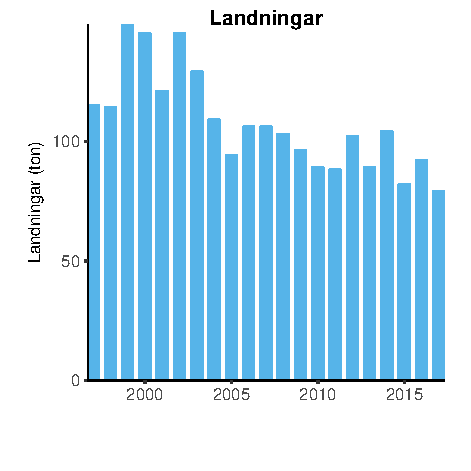
\includegraphics{Making_figures_for_RoM_in_R_files/figure-latex/unnamed-chunk-15-1} 

}

\caption{Gädda in the "Great Lakes" (RoM 2018) - example of a single-series plot using R}\label{fig:unnamed-chunk-15}
\end{figure}

Save the file (to your working directory)

\begin{Shaded}
\begin{Highlighting}[]
\KeywordTok{ggsave}\NormalTok{(}\StringTok{"Fig_1.tiff"}\NormalTok{, }\DataTypeTok{plot =}\NormalTok{ p1, }\DataTypeTok{dpi =} \DecValTok{300}\NormalTok{, }\DataTypeTok{width =} \DecValTok{8}\NormalTok{, }\DataTypeTok{height =} \DecValTok{8}\NormalTok{, }\DataTypeTok{units =} \StringTok{"cm"}\NormalTok{)}
\end{Highlighting}
\end{Shaded}

\subsection{Fig. 2. Multiple series}\label{fig.-2.-multiple-series}

\begin{figure}

{\centering 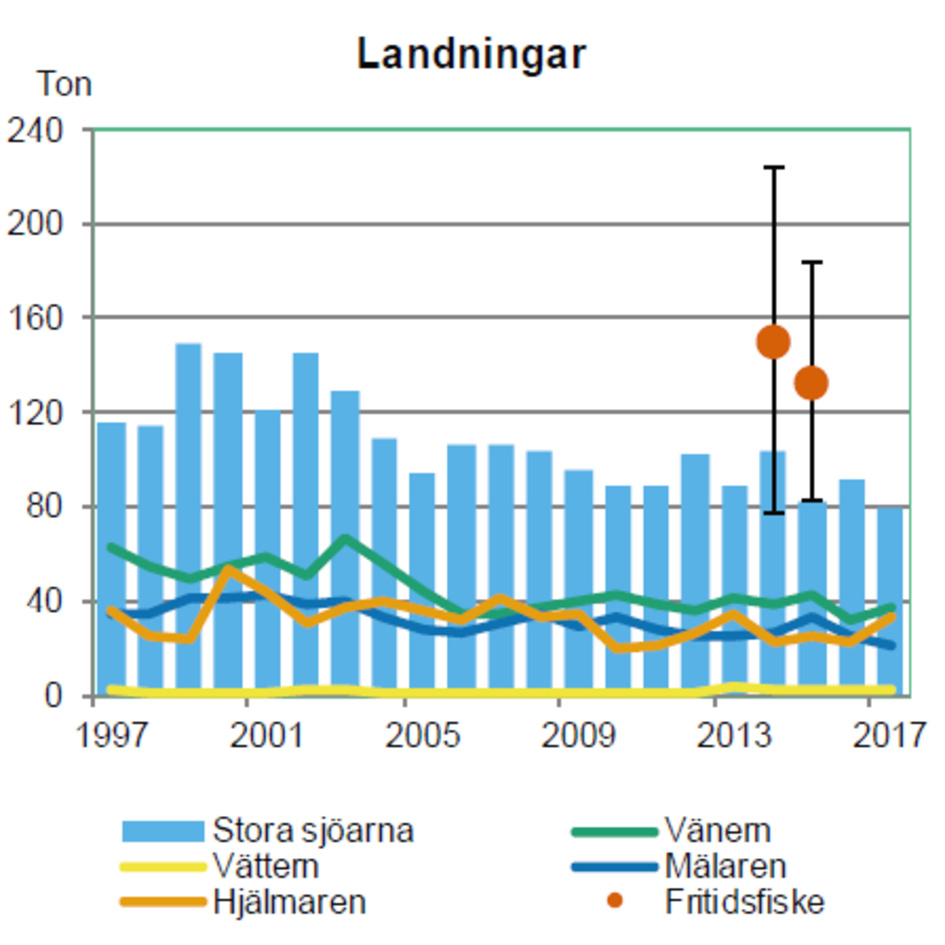
\includegraphics{gadda} 

}

\caption{Gädda in the "Great Lakes" (RoM 2018) - example of a multiple-series plot}\label{fig:unnamed-chunk-17}
\end{figure}

We now need to specify y-axis titles and plot title, and in addition we
need to define how mnay levels we have! For the pike data we can set
them as:

\begin{Shaded}
\begin{Highlighting}[]
\NormalTok{y_axis <-}\StringTok{ }\KeywordTok{c}\NormalTok{(}\StringTok{"Landningar (ton)"}\NormalTok{)}
\NormalTok{title <-}\StringTok{ }\KeywordTok{c}\NormalTok{(}\StringTok{"Landningar"}\NormalTok{) }
\NormalTok{main_series <-}\StringTok{ }\KeywordTok{c}\NormalTok{(}\StringTok{"Stora sjöarna"}\NormalTok{)}
\NormalTok{n_lev <-}\StringTok{ }\KeywordTok{length}\NormalTok{(}\KeywordTok{unique}\NormalTok{(dat}\OperatorTok{$}\NormalTok{Område)) }
\NormalTok{special_series <-}\StringTok{ }\KeywordTok{c}\NormalTok{(}\StringTok{"Fritidsfiske"}\NormalTok{)}
\end{Highlighting}
\end{Shaded}

Note that we in this example use multiple data series, and that one of
them is is recreational fisheries that in turn has error bars.
\textbf{These need to be in columns, so that we have a high (rec\_plus)
and a low (rec\_minu) column. Note also that they are NA when the Område
is not equal to recreational fisheries}

\begin{Shaded}
\begin{Highlighting}[]
\KeywordTok{head}\NormalTok{(dat) }
\end{Highlighting}
\end{Shaded}

\begin{verbatim}
##     År error rec_plus rec_minu        Område Ton
## 1 1997    NA       NA       NA Stora sjöarna 115
## 2 1998    NA       NA       NA Stora sjöarna 114
## 3 1999    NA       NA       NA Stora sjöarna 149
## 4 2000    NA       NA       NA Stora sjöarna 145
## 5 2001    NA       NA       NA Stora sjöarna 121
## 6 2002    NA       NA       NA Stora sjöarna 145
\end{verbatim}

\begin{Shaded}
\begin{Highlighting}[]
\KeywordTok{tail}\NormalTok{(dat)}
\end{Highlighting}
\end{Shaded}

\begin{verbatim}
##       År error rec_plus rec_minu       Område Ton
## 121 2012    NA       NA       NA Fritidsfiske  NA
## 122 2013    NA       NA       NA Fritidsfiske  NA
## 123 2014    73      223       77 Fritidsfiske 150
## 124 2015    51      184       82 Fritidsfiske 133
## 125 2016    NA       NA       NA Fritidsfiske  NA
## 126 2017    NA       NA       NA Fritidsfiske  NA
\end{verbatim}

\begin{Shaded}
\begin{Highlighting}[]
\NormalTok{p2 <-}\StringTok{ }\KeywordTok{ggplot}\NormalTok{(dat, }\KeywordTok{aes}\NormalTok{(År, Ton, }\DataTypeTok{color =}\NormalTok{ Område)) }\OperatorTok{+}
\StringTok{  }\KeywordTok{geom_bar}\NormalTok{(}\DataTypeTok{data =} \KeywordTok{subset}\NormalTok{(dat, Område }\OperatorTok{==}\StringTok{ }\NormalTok{main_series), }
           \KeywordTok{aes}\NormalTok{(}\DataTypeTok{x =}\NormalTok{ År, }\DataTypeTok{y =}\NormalTok{ Ton), }\DataTypeTok{stat =} \StringTok{"identity"}\NormalTok{, }\DataTypeTok{color =}\NormalTok{ pal[}\DecValTok{1}\NormalTok{], }\DataTypeTok{fill =}\NormalTok{ pal[}\DecValTok{1}\NormalTok{], }
           \DataTypeTok{width =} \FloatTok{0.6}\NormalTok{) }\OperatorTok{+}
\StringTok{  }\KeywordTok{geom_line}\NormalTok{(}\DataTypeTok{data =}\NormalTok{ dat, }\KeywordTok{aes}\NormalTok{(År, Ton, }\DataTypeTok{color =}\NormalTok{ Område, }\DataTypeTok{alpha =}\NormalTok{ Område), }
            \DataTypeTok{size =} \DecValTok{1}\NormalTok{) }\OperatorTok{+}\StringTok{ }
\StringTok{  }\KeywordTok{geom_point}\NormalTok{(}\DataTypeTok{data =} \KeywordTok{subset}\NormalTok{(dat, Område }\OperatorTok{==}\StringTok{ }\NormalTok{special_series), }\CommentTok{# here we define our special series}
             \KeywordTok{aes}\NormalTok{(År, Ton, }\DataTypeTok{fill =}\NormalTok{ Område), }\DataTypeTok{size =} \DecValTok{2}\NormalTok{, }\DataTypeTok{color =}\NormalTok{ pal[}\KeywordTok{max}\NormalTok{(n_lev)]) }\OperatorTok{+}\StringTok{ }
\StringTok{  }\CommentTok{# above the number of level enters (max(n_lev))}
\StringTok{  }\KeywordTok{geom_errorbar}\NormalTok{(}\DataTypeTok{data =} \KeywordTok{subset}\NormalTok{(dat, Område }\OperatorTok{==}\StringTok{ }\NormalTok{special_series), }
                \KeywordTok{aes}\NormalTok{(}\DataTypeTok{x =}\NormalTok{ År, }\DataTypeTok{ymin =}\NormalTok{ rec_minu, }\DataTypeTok{ymax =}\NormalTok{ rec_plus), }
                \DataTypeTok{show.legend =} \OtherTok{FALSE}\NormalTok{, }\DataTypeTok{width  =} \DecValTok{1}\NormalTok{, }\DataTypeTok{color =}\NormalTok{ pal[}\KeywordTok{max}\NormalTok{(n_lev)]) }\OperatorTok{+}
\StringTok{  }\KeywordTok{scale_color_manual}\NormalTok{(}\DataTypeTok{values =}\NormalTok{ pal[}\KeywordTok{seq}\NormalTok{(}\DecValTok{1}\NormalTok{, n_lev)]) }\OperatorTok{+}
\StringTok{  }\KeywordTok{scale_alpha_manual}\NormalTok{(}\DataTypeTok{values =} \KeywordTok{c}\NormalTok{(}\KeywordTok{rep}\NormalTok{(}\DecValTok{1}\NormalTok{, (n_lev}\OperatorTok{-}\DecValTok{1}\NormalTok{)), }\DecValTok{0}\NormalTok{)) }\OperatorTok{+}\StringTok{ }
\StringTok{  }\CommentTok{# above we set the line between rec fisheries transparent}
\StringTok{  }\KeywordTok{labs}\NormalTok{(}\DataTypeTok{x =} \StringTok{""}\NormalTok{, }\DataTypeTok{y =}\NormalTok{ y_axis) }\OperatorTok{+}
\StringTok{  }\KeywordTok{ggtitle}\NormalTok{(title) }\OperatorTok{+}
\StringTok{  }\KeywordTok{guides}\NormalTok{(}\DataTypeTok{fill  =} \OtherTok{FALSE}\NormalTok{,}
         \DataTypeTok{alpha =} \OtherTok{FALSE}\NormalTok{,}
         \DataTypeTok{color =} \KeywordTok{guide_legend}\NormalTok{(}\DataTypeTok{nrow =} \DecValTok{3}\NormalTok{, }
                              \DataTypeTok{title =} \StringTok{""}\NormalTok{,}
                              \DataTypeTok{override.aes =} \KeywordTok{list}\NormalTok{(}\DataTypeTok{size =} \FloatTok{1.3}\NormalTok{, }
                                                  \DataTypeTok{color =}\NormalTok{ pal[}\KeywordTok{seq}\NormalTok{(}\DecValTok{1}\NormalTok{, n_lev)]),}
                              \DataTypeTok{keywidth =} \FloatTok{0.3}\NormalTok{,}
                              \DataTypeTok{keyheight =} \FloatTok{0.1}\NormalTok{,}
                              \DataTypeTok{default.unit =} \StringTok{"inch"}\NormalTok{)) }\OperatorTok{+}
\StringTok{  }\KeywordTok{scale_x_continuous}\NormalTok{(}\DataTypeTok{expand =} \KeywordTok{c}\NormalTok{(}\DecValTok{0}\NormalTok{, }\DecValTok{0}\NormalTok{), }\DataTypeTok{breaks =}\NormalTok{ scales}\OperatorTok{::}\KeywordTok{pretty_breaks}\NormalTok{(}\DataTypeTok{n =} \DecValTok{6}\NormalTok{)) }\OperatorTok{+}
\StringTok{  }\KeywordTok{scale_y_continuous}\NormalTok{(}\DataTypeTok{expand =} \KeywordTok{c}\NormalTok{(}\DecValTok{0}\NormalTok{, }\DecValTok{0}\NormalTok{), }\DataTypeTok{breaks =}\NormalTok{ scales}\OperatorTok{::}\KeywordTok{pretty_breaks}\NormalTok{(}\DataTypeTok{n =} \DecValTok{5}\NormalTok{)) }\OperatorTok{+}
\StringTok{  }\KeywordTok{theme_rom}\NormalTok{()}
\end{Highlighting}
\end{Shaded}

\begin{figure}

{\centering 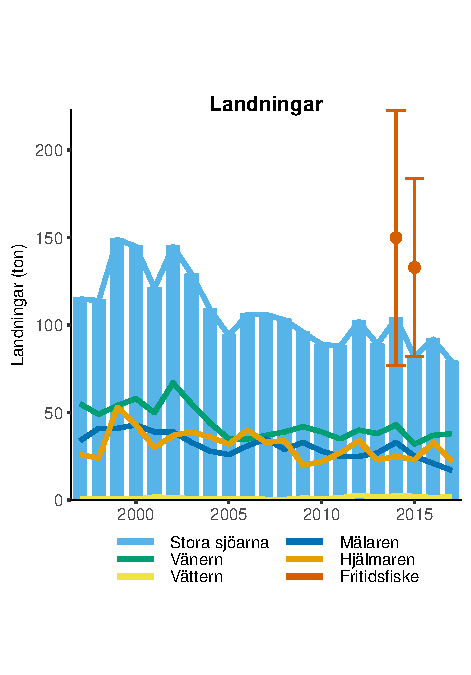
\includegraphics{Making_figures_for_RoM_in_R_files/figure-latex/unnamed-chunk-21-1} 

}

\caption{Gädda in the Great Lakes (RoM 2018) - example of a multiple-series plot using R}\label{fig:unnamed-chunk-21}
\end{figure}

Now save the file (to your working directory)

\begin{Shaded}
\begin{Highlighting}[]
\KeywordTok{ggsave}\NormalTok{(}\StringTok{"Fig_2.tiff"}\NormalTok{, }\DataTypeTok{plot =}\NormalTok{ p2, }\DataTypeTok{dpi =} \DecValTok{300}\NormalTok{, }\DataTypeTok{width =} \DecValTok{8}\NormalTok{, }\DataTypeTok{height =} \DecValTok{8}\NormalTok{, }\DataTypeTok{units =} \StringTok{"cm"}\NormalTok{)}
\end{Highlighting}
\end{Shaded}

Let's say that you have 3 different areas and no special series and no
error bars. Then you simply need to hashtag the code the plots those
features. We subset the full data as an example:

\begin{Shaded}
\begin{Highlighting}[]
\NormalTok{dat2 <-}\StringTok{ }\NormalTok{dat }\OperatorTok\StringTok{ }
\StringTok{  }\KeywordTok{select}\NormalTok{(År, Ton, Område) }\OperatorTok\StringTok{ }
\StringTok{  }\KeywordTok{filter}\NormalTok{(Område }\OperatorTok\StringTok{ }\KeywordTok{c}\NormalTok{(}\StringTok{"Stora sjöarna"}\NormalTok{, }\StringTok{"Mälaren"}\NormalTok{))}
\end{Highlighting}
\end{Shaded}

We now need to update the number of levels in the data:

\begin{Shaded}
\begin{Highlighting}[]
\NormalTok{n_lev <-}\StringTok{ }\KeywordTok{length}\NormalTok{(}\KeywordTok{unique}\NormalTok{(dat2}\OperatorTok{$}\NormalTok{Område)) }
\end{Highlighting}
\end{Shaded}

Repeat the general Fig. 2 plot, but remove the points and errorbars:

\begin{Shaded}
\begin{Highlighting}[]
\NormalTok{p2a <-}\StringTok{ }\KeywordTok{ggplot}\NormalTok{(dat2, }\KeywordTok{aes}\NormalTok{(År, Ton, }\DataTypeTok{color =}\NormalTok{ Område)) }\OperatorTok{+}
\StringTok{  }\KeywordTok{geom_bar}\NormalTok{(}\DataTypeTok{data =} \KeywordTok{subset}\NormalTok{(dat2, Område }\OperatorTok{==}\StringTok{ }\NormalTok{main_series), }
           \KeywordTok{aes}\NormalTok{(}\DataTypeTok{x =}\NormalTok{ År, }\DataTypeTok{y =}\NormalTok{ Ton), }\DataTypeTok{stat =} \StringTok{"identity"}\NormalTok{, }\DataTypeTok{color =}\NormalTok{ pal[}\DecValTok{1}\NormalTok{], }\DataTypeTok{fill =}\NormalTok{ pal[}\DecValTok{1}\NormalTok{], }
           \DataTypeTok{width =} \FloatTok{0.6}\NormalTok{) }\OperatorTok{+}
\StringTok{  }\KeywordTok{geom_line}\NormalTok{(}\DataTypeTok{data =}\NormalTok{ dat2, }\KeywordTok{aes}\NormalTok{(År, Ton, }\DataTypeTok{color =}\NormalTok{ Område, }\DataTypeTok{alpha =}\NormalTok{ Område), }
            \DataTypeTok{size =} \DecValTok{1}\NormalTok{) }\OperatorTok{+}\StringTok{ }
\StringTok{  }\CommentTok{#geom_point(data = subset(dat, Område == special_series), # here we define our special series}
\StringTok{  }\CommentTok{#           aes(År, Ton, fill = Område), size = 2, color = pal[max(n_lev)]) + }
\StringTok{  }\CommentTok{#geom_errorbar(data = subset(dat, Område == special_series), }
\StringTok{  }\CommentTok{#              aes(x = År, ymin = rec_minu, ymax = rec_plus), }
\StringTok{  }\CommentTok{#              show.legend = FALSE, width  = 1, color = pal[max(n_lev)]) +}
\StringTok{  }\KeywordTok{scale_color_manual}\NormalTok{(}\DataTypeTok{values =}\NormalTok{ pal[}\KeywordTok{seq}\NormalTok{(}\DecValTok{1}\NormalTok{, n_lev)]) }\OperatorTok{+}
\StringTok{  }\CommentTok{#scale_alpha_manual(values = c(rep(1, (n_lev-1)), 0)) + }
\StringTok{  }\KeywordTok{labs}\NormalTok{(}\DataTypeTok{x =} \StringTok{""}\NormalTok{, }\DataTypeTok{y =}\NormalTok{ y_axis) }\OperatorTok{+}
\StringTok{  }\KeywordTok{ggtitle}\NormalTok{(title) }\OperatorTok{+}
\StringTok{  }\KeywordTok{guides}\NormalTok{(}\DataTypeTok{fill  =} \OtherTok{FALSE}\NormalTok{,}
         \DataTypeTok{alpha =} \OtherTok{FALSE}\NormalTok{,}
         \DataTypeTok{color =} \KeywordTok{guide_legend}\NormalTok{(}\DataTypeTok{nrow =} \DecValTok{3}\NormalTok{, }
                              \DataTypeTok{title =} \StringTok{""}\NormalTok{,}
                              \DataTypeTok{override.aes =} \KeywordTok{list}\NormalTok{(}\DataTypeTok{size =} \FloatTok{1.3}\NormalTok{, }
                                                  \DataTypeTok{color =}\NormalTok{ pal[}\KeywordTok{seq}\NormalTok{(}\DecValTok{1}\NormalTok{, n_lev)]),}
                              \DataTypeTok{keywidth =} \FloatTok{0.3}\NormalTok{,}
                              \DataTypeTok{keyheight =} \FloatTok{0.1}\NormalTok{,}
                              \DataTypeTok{default.unit =} \StringTok{"inch"}\NormalTok{)) }\OperatorTok{+}
\StringTok{  }\KeywordTok{scale_x_continuous}\NormalTok{(}\DataTypeTok{expand =} \KeywordTok{c}\NormalTok{(}\DecValTok{0}\NormalTok{, }\DecValTok{0}\NormalTok{), }\DataTypeTok{breaks =}\NormalTok{ scales}\OperatorTok{::}\KeywordTok{pretty_breaks}\NormalTok{(}\DataTypeTok{n =} \DecValTok{6}\NormalTok{)) }\OperatorTok{+}
\StringTok{  }\KeywordTok{scale_y_continuous}\NormalTok{(}\DataTypeTok{expand =} \KeywordTok{c}\NormalTok{(}\DecValTok{0}\NormalTok{, }\DecValTok{0}\NormalTok{), }\DataTypeTok{breaks =}\NormalTok{ scales}\OperatorTok{::}\KeywordTok{pretty_breaks}\NormalTok{(}\DataTypeTok{n =} \DecValTok{5}\NormalTok{)) }\OperatorTok{+}
\StringTok{  }\KeywordTok{theme_rom}\NormalTok{()}
\end{Highlighting}
\end{Shaded}

\begin{figure}

{\centering 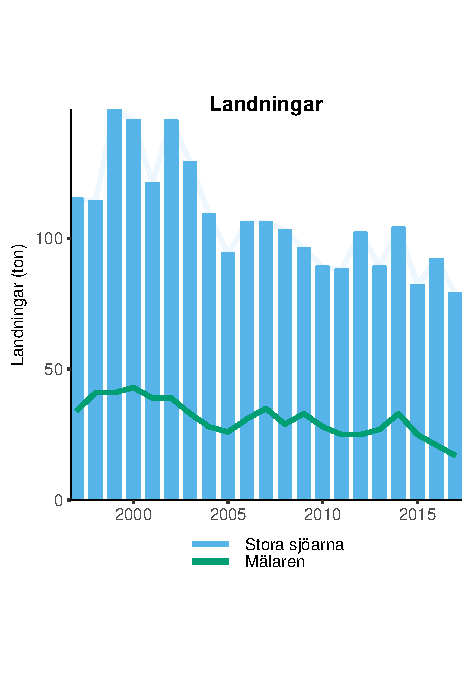
\includegraphics{Making_figures_for_RoM_in_R_files/figure-latex/unnamed-chunk-26-1} 

}

\caption{Gädda in the Great Lakes (RoM 2018) - example of a multiple-series plot using R}\label{fig:unnamed-chunk-26}
\end{figure}

\subsubsection{To work on:}\label{to-work-on}

\begin{itemize}
\item
  secondary y-axis that is not a one-to-one transformation of the
  primary axes. Possible?
\item
  set Ton in column name as biomass and define ton as a vector!
\item
  name chunks
\item
  write comments in pdf: what about aspect ratio?
\end{itemize}


\end{document}
